This chapter outlines the reconstruction of the physics objects used in the ATLAS experiment. The object selection criteria employed in the $VH(WW^{*})$ analysis will be presented in the next chapter. The analysis makes use of \met{}, electrons, muons, and jets, all of which are reconstructed in the events. Photons are not used in this analysis and are therefore omitted from the discussion, but can be read about in~\cite{ATLAS:2019qmc}. Taus that decay hadronically are not explicitly reconstructed, while leptonically decaying taus may be identified as electrons or muons and are thus implicitly included through the lepton channels. Figure~\ref{fig:reco_atlas_particles} illustrates what different particles look like when passing through the ATLAS detector.

\begin{figure}[hpt]
  \centering
  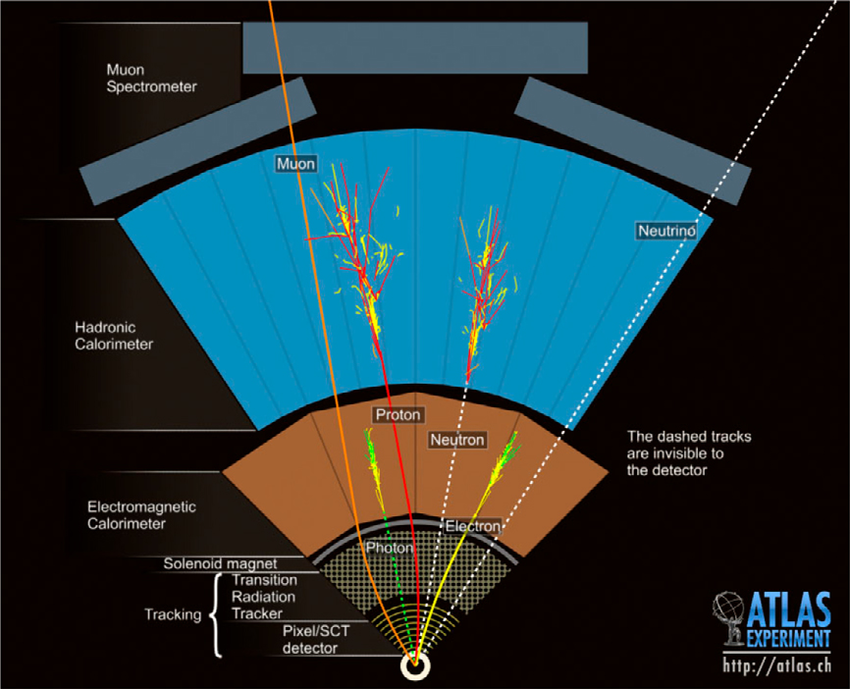
\includegraphics[width=0.55\textwidth]{figures/reco/reco_atlas_particles.png}
  \caption{Illustration of the different particles reconstructed in the ATLAS detector. The particles are shown as they would appear in the ATLAS detector, with their corresponding reconstructed objects. Taken from~\cite{reco_particles}.}\label{fig:reco_atlas_particles}
\end{figure}